\documentclass{standalone}
\usepackage{tikz}
\usepackage{pgfmath} % use to create randum numbers


\begin{document}
\usetikzlibrary{math} %needed tikz library

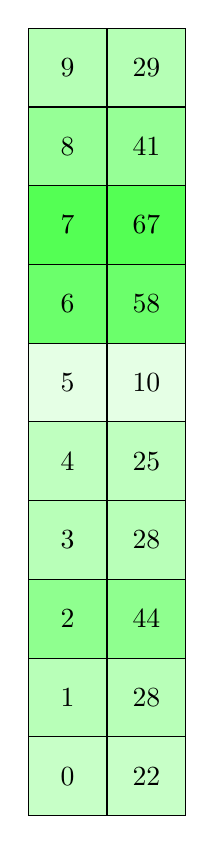
\begin{tikzpicture}[block/.style={rectangle, draw, minimum size=1cm}]

% Create ten boxes
\foreach \i in {0,...,9} {
    % Create ten random numbers between i and 100 and store the value in variable `vara`
    \pgfmathparse{int(random(\i,100))}\let\vara=\pgfmathresult 

    % seeding ensures we have a random set of numbers everytime
    \pgfmathsetseed{\i}

    % Heres the labels
    \node[block, fill = green!\vara ] at (1,\i) {$\vara$};
    \node[block, fill = green!\vara ] at (0,\i + 0) {$ \i$};

    % and the subscripts
    % \node[below] at (0.25,\i + .25) {$\i$};
}
\end{tikzpicture}
\end{document}